% -----------------------------------------------------------------
%        File: thesis.tex
% Description: Thesis
%      Author: Andrew Parlane
% -----------------------------------------------------------------

% This file is part of https://github.com/andrewparlane/fiuba_thesis
% Copyright (c) 2022 Andrew Parlane.
%
% This is free software: you can redistribute it and/or modify it under
% the terms of the GNU General Public License as published by the Free
% Software Foundation, version 3.
%
% This program is distributed in the hope that it will be useful, but
% WITHOUT ANY WARRANTY; without even the implied warranty of
% MERCHANTABILITY or FITNESS FOR A PARTICULAR PURPOSE. See the GNU
% General Public License for more details.
%
% You should have received a copy of the GNU General Public License
% along with this code. If not, see <http://www.gnu.org/licenses/>.

% Note: This thesis was written and compiled using overleaf
%       Building it via pdflatex has been tested, but not extensively

\documentclass[a4paper, twoside, 11pt]{report}

% =============================================
% Includes
% =============================================

% packages
% -----------------------------------------------------------------
%        File: packages.tex
% Description: Various packages
%      Author: Andrew Parlane
% -----------------------------------------------------------------

% This file is part of https://github.com/andrewparlane/fiuba_thesis
% Copyright (c) 2022 Andrew Parlane.
%
% This is free software: you can redistribute it and/or modify it under
% the terms of the GNU General Public License as published by the Free
% Software Foundation, version 3.
%
% This program is distributed in the hope that it will be useful, but
% WITHOUT ANY WARRANTY; without even the implied warranty of
% MERCHANTABILITY or FITNESS FOR A PARTICULAR PURPOSE. See the GNU
% General Public License for more details.
%
% You should have received a copy of the GNU General Public License
% along with this code. If not, see <http://www.gnu.org/licenses/>.

% Maths stuff (\begin{align*} for one)
\usepackage{amsmath}

% Spanish Localisation
\usepackage[spanish]{babel}

% UTF8 encoding allows for accents. Must come before biblatex
\usepackage[utf8]{inputenc}

% Bibliography
\usepackage[backend=biber, style=numeric]{biblatex}

% For \captionsetup
\usepackage{caption}

% Required by biblatex and must come after inputenc
\usepackage{csquotes}

% dirtree (for outputting the dir tree of the repos)
\usepackage{dirtree}

% Better lists, allows setting \parsep
\usepackage{enumitem}

% A4 + default margins
\usepackage[a4paper]{geometry}

% Images
\usepackage{graphicx}

% For embedding code
\usepackage{listings}

% Multirow
\usepackage{multirow}

% for \nicefrac
\usepackage{nicefrac}

% For \onehalfspacing
\usepackage{setspace}

% For \FloatBarrier
\usepackage{placeins}

% SI Units
\usepackage{siunitx}

% Allows for setting space between sections
\usepackage[compact]{titlesec}

% Links (must be loaded after titlesec)
\usepackage{hyperref}

% Fix links to images so they actually show the image
\usepackage[all]{hypcap}

% TabularY (for autosizing columns (L) in the port list tabels)
\usepackage{tabulary}

% Change spacing around ToC
\usepackage{tocloft}

% Colours for table row zebras
\usepackage[table]{xcolor}


% settings
% -----------------------------------------------------------------
%        File: settings.tex
% Description: Various configuration settings
%      Author: Andrew Parlane
% -----------------------------------------------------------------

% This file is part of https://github.com/andrewparlane/fiuba_thesis
% Copyright (c) 2022 Andrew Parlane.
%
% This is free software: you can redistribute it and/or modify it under
% the terms of the GNU General Public License as published by the Free
% Software Foundation, version 3.
%
% This program is distributed in the hope that it will be useful, but
% WITHOUT ANY WARRANTY; without even the implied warranty of
% MERCHANTABILITY or FITNESS FOR A PARTICULAR PURPOSE. See the GNU
% General Public License for more details.
%
% You should have received a copy of the GNU General Public License
% along with this code. If not, see <http://www.gnu.org/licenses/>.


% Don't indent paragraphs
\setlength{\parindent}{0cm}

% Space between paragraphs
\parskip 1.5ex

% Line spacing: 1.5
\onehalfspacing

% Reduce space between items in \begin{description}, \begin{itemize} and \begin{enumerate}
\setlist[description]{noitemsep, nolistsep, topsep=0pt}
\setlist[itemize]{noitemsep, nolistsep, topsep=0pt}
\setlist[enumerate]{noitemsep, nolistsep, topsep=0pt}

% Change Table of Contents name from "Índice General" to "Índice"
\addto\captionsspanish{
  \renewcommand{\contentsname}
    {Índice}
}

% \Chapter format - Huge, bold, no numbering
\titleformat{\chapter}{\normalfont\Huge\bfseries}{}{0pt}{}

% Reduce space before and after the \chapter title
\titlespacing{\chapter}{0pt}{-1em}{1em}

% \Section format - huge, bold
\titleformat{\section}{\normalfont\huge\bfseries}{\thesection}{0pt}{}

% \Subsection format - LARGE, bold
\titleformat{\subsection}{\normalfont\LARGE\bfseries}{\thesection}{0pt}{}

% \subsubsection format - Large
\titleformat{\subsubsection}{\normalfont\Large}{\thesection}{0pt}{}

% Don't number sections
\setcounter{secnumdepth}{0}

% Sets links to blue
\hypersetup{
    colorlinks,
    citecolor=blue,
    filecolor=blue,
    linkcolor=blue,
    urlcolor=blue
}

% ToC depth to \subsubsection
\setcounter{tocdepth}{3}

% Remove spacing at top of page before and after the Índice title
\setlength{\cftbeforetoctitleskip}{0pt}
\setlength{\cftaftertoctitleskip}{0pt}

% Don't hyphonate over pages
\brokenpenalty10000\relax

% Captions should "hang" aka align with the start, and not with the label
\captionsetup{format=hang}

% Create a new command for referencing figures with "Figura ?.?" as the link. Same for tables and sections
% Call with:
%  \figref{fig:figure-label} 
%  \tabref{tab:table-label}
%  \secref{sec:section-label}{Section Name}
\newcommand*{\figref}[1]{\hyperref[#1]{Figura~\ref*{#1}}}
\newcommand*{\tabref}[1]{\hyperref[#1]{Cuadro~\ref*{#1}}}
\newcommand*{\secref}[2]{\hyperref[#1]{Sección #2}}

% Zebra pattern in tables
\newcommand*{\tablezebra}{\rowcolors{2}{white}{lightgray!35}}

% Let's us restart the row num to reset the zebra pattern using \setcounter{rownum}{0}
\makeatletter
\@ifundefined{c@rownum}{\let\c@rownum\rownum}{}
\makeatother


% Bibliography
\addbibresource{bibliography.bib}

% =============================================
% Document
% =============================================

\begin{document}

% ---------------------------------------------
% Title Page
% ---------------------------------------------
\begin{titlepage}

\capstartfalse
\begin{figure}
\centering
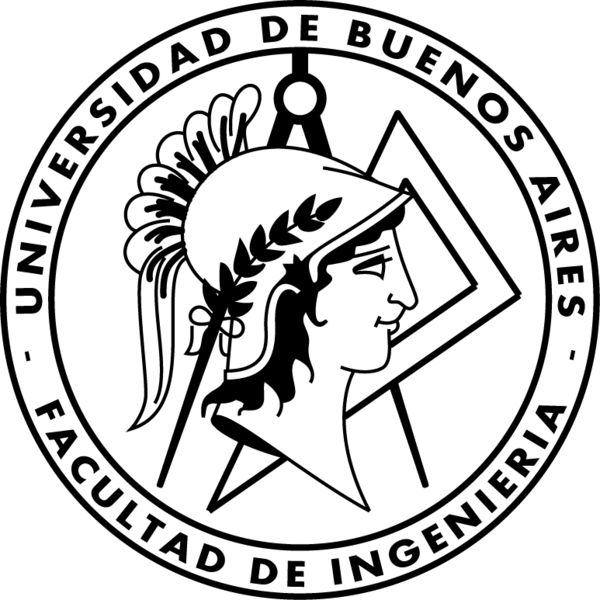
\includegraphics[scale=1.7]{./img/logo-facu.png}
\end{figure}
\capstarttrue

\begin{center}
    \Large{Universidad de Buenos Aires} \\
    \Large{Facultad de Ingeniería} \\
    \Large{Tesis de Maestría en Ciencias de la Ingeniería} \\
    \vspace{5mm}
    \huge{\bf Desarrollo de circuitos integrados CMOS para aplicaciones de RFID} \\
    \vspace{8mm}
    \huge{\bf Andrew Parlane}
\end{center}

\vspace*{\fill}

\begin{description}
    \item[\large{Director:}] \hspace{21pt} \large{Dr. Ing. Mariano Garcia-Inza}
    \item[\large{Codirectores:}] \large{Ing. Federico G. Zacchigna, Ing. Octavio Alpago}
\end{description}
\end{titlepage}

% ---------------------------------------------
% Resumen
% ---------------------------------------------

\FloatBarrier
%\chapter* so it doesn't get added to the ToC
\chapter*{Resumen}
Este trabajo presenta el diseño de circuitos integrados digitales para la implementación de un TAG RFID en un chip CMOS. Los requerimientos de los circuitos son definidos por un proyecto de investigación marco cuyo objetivo general es el desarrollo de sensores inalámbricos de radiación ionizante para dosimetría médica. Esto requiere la integración de diferentes subsistemas en un ASIC a fabricar en tecnología CMOS.

Los circuitos presentados en esta tesis consisten en un bloque digital de control, que puede recibir y responder a las tramas definidas en la norma ISO/IEC 14443A, y mediante un protocolo propietario encima de la norma, controlar otros subcircuitos del chip necesarios para la adquisición de la señal dosimétrica y su posterior transmisión inalámbrica. La implementación de la norma es presentada en un núcleo IP genérico. Por lo tanto es apto para uso en otros proyectos y con cualquier lector comercial que trabaje bajo norma. El protocolo propietario consiste en cinco mensajes que permiten el muestreo de hasta quince TAGs de forma sincronizada. El muestreo simultáneo de múltiples TAGs sensores utilizando RFID es una estrategia novedosa desarrollada en esta tesis, el cual representa un potencial avance en el desarrollo de métodos de control dosimétrico en aplicaciones médicas.

El trabajo realizado incluye el diseño de los bloques digitales utilizando HDL SystemVerilog y su verificación funcional. Luego, se utiliza el kit de diseño del proceso (PDK, por sus siglas en Inglés) XH018 (nodo tecnológico de \SI{180}{\nano\meter}) de la foundry XFAB para realizar la síntesis, el place and route y la generación de las máscaras de fabricación (layout).

Las pruebas de verificación llevadas a cabo dan alta confianza en el diseño. Las mismas incluyen: más de cien horas de simulaciones del RTL ejecutando 187 aserciones de SystemVerilog más de cien mil millones de veces y generando informes de cobertura de código, la verificación formal de equivalencia entre lógica RTL y los netlists post síntesis y post implementación, Design Rules Check (DRC), y Layout Vs Schematic (LVS); todas esas pruebas tienen resultados favorables.

El layout final no tiene violaciones de timing, el slack de Setup menor es \SI{1,59}{\nano\second} y de Hold es \SI{0,02}{\nano\second}, el área utilizada es \SI{0,087}{\milli\meter\squared} (\SI{295,68}{\micro\meter} por \SI{294,00}{\micro\meter}), y la estimación de consumo de potencia promedio es \SI{256}{\micro\watt}.

% ---------------------------------------------
% Aclaraciones
% ---------------------------------------------

\FloatBarrier
%\chapter* so it's not in the ToC
\chapter*{Aclaraciones}

Aclaraciones
Por cuestiones de claridad en esta tesis cuándo se dice que una señal está en ‘1’ o ‘0’ significa que la señal tiene un valor lógico igual a '1' o ‘0’ respectivamente.

El código RTL, los bancos de pruebas y los scripts de síntesis y place \& route están publicados de forma abierta en GitHub bajo la licencia GNU v3.0, de manera que cualquier parte de este trabajo pueda ser utilizada en otros proyectos académicos o comerciales. Para facilitar la adopción y modificación de este trabajo por la comunidad internacional, el código y los scripts están escritos con nombres y comentarios en Inglés.

Para facilitar la lectura de esta tesis las señales, variables y parámetros están escritos en \textit{cursiva},  los módulos, clases y funciones están escritos en \textbf{negritas}. Además se utilizan paréntesis para nombrar a las funciones, aunque sin sus argumentos, por ejemplo: \textbf{compare()}. Finalmente los nombres de las tramas definidas en los protocolos están escritos en MAYÚSCULAS.

% ---------------------------------------------
% TOC
% ---------------------------------------------
\newpage
\tableofcontents

% ---------------------------------------------
% Introducción
% ---------------------------------------------

\FloatBarrier
\chapter{Introducción}

% Motivación y Contexto de Trabajo
% --------------------------------
\FloatBarrier
\section{Motivación y Contexto de Trabajo}

La radioterapia es un tratamiento médico que consiste en utilizar radiación ionizante para eliminar células cancerígenas que forman tumores. Sin embargo, la radiación puede presentar riesgos a tejido sano, especialmente si la dosis aplicada es mayor a la necesaria o mal localizada. Hay varios incidentes registrados donde algunas personas recibieron una sobredosis durante radioterapia, y en algunos casos dosis letales~\cite{UNSE_2019}. Por otro lado, una dosis localizada pero demasiado pequeña reduciría la efectividad del tratamiento. Por esas razones es muy importante adoptar consideraciones de QA (Quality Assurance), la cual puede definirse como:

\begin{displaycquote}[traducción mía]{qa_in_radiotherapy}
Los procedimientos que aseguren el cumplimiento de las prescripciones médicas con respeto a la dosis entregada al volumen deseado, junto con una dosis mínima a tejido sano, exposición mínima al personal, y el monitoreo adecuado del paciente para determinar el resultado del tratamiento.
\end{displaycquote}

Una técnica importante en QA es dosimetría in-vivo (IVD), que es la práctica de medir la dosis recibida durante el tratamiento en tiempo real. La IVD es recomendada para su uso en radioterapia~\cite{AAPM-1994}\cite{ICRP-2000}, con un error menor del 3\% por tratamiento. Existen varios tipos de sensores de radiación que pueden ser utilizados en IVD con radioterapia. Entre ellos se encuentran los sensores MOSFET, los cuales tienen varias ventajas, como por ejemplo que pueden ser leídos en tiempo real o posteriormente, son pequeños y robustos, pero también tienen algunas limitaciones~\cite{UNSE_2019}. Los investigadores del Laboratorio de Física de Dispositivos - Microelectrónica de la Facultad de Ingeniería de la Universidad de Buenos Aires han trabajando durante los últimos años en mejorar el desempeño de sensores MOSFET de radiación para uso en IVD~\cite{mosfet_mismatch_amplification}\cite{6MV_LINAC}. Otra ventaja de los sensores MOSFETs es que pueden ser integrados en un mismo chip con circuitos adicionales que permitan su lectura, digitalización y posterior transmisión de los resultados en tiempo real. Esto representa una importante ventaja frente al método usual de lectura post irradiación, ya que el seguimiento en tiempo real permitiría ajustar la dosis durante la ejecución del tratamiento.

Un sensor pequeño construido con una cantidad mínima de componentes permitiría obtener arreglos de sensores con excelente resolución espacial y así realizar un mapeo dosimétrico de una zona de interés. A la hora de implementar esta solución, los TAGs RFID (Radio Frequency Identification) pasivos son una excelente opción, ya que sólo requieren del circuito integrado y una antena externa. La alimentación y la comunicación pueden realizarse a través del campo electromagnético generado por el dispositivo de lectura. Un sistema de estas características, además de ser más simple, sería más cómodo para el paciente y más práctico para su uso en el campo médico.

En su tesis de 2018~\cite{Arana_thesis}, Arana analizó la relación entre la frecuencia de operación de un TAG RFID y su distancia máxima de la lectura considerando los límites de exposición de humanos a campos electromagnéticos definidos en IEEE C95.1. Los resultados muestran que una frecuencia en el orden de 10 MHz daría el mejor rango de operación mientras manteniendo el campo electromagnético (EM) dentro de límites seguros. Esta frecuencia se encuentra cercana a los 13.56 MHz de RFID HF (High Frequency). Arana muestra en su tesis el diseño de la antena y de circuitos integrados analógicos para un TAG ISO/IEC 14443 tipo A que puede funcionar a una distancia de 30 cm de la lectura. También en una publicación de 2014~\cite{fabricio_eamta}, Alcalde et al. presentan el diseño y fabricación de un TAG RFID que implementa parte de la norma ISO/IEC 14443 tipo A. El funcionamiento es verificado a través de mediciones experimentales del sistema funcionando en loopback.

Un atributo del protocolo ISO/IEC 14443A es que permite hasta 15 TAGs activos al mismo tiempo. Esto da la posibilidad de obtener muestras de los sensores de forma sincronizada, con la ventaja de medir en múltiples lugares del cuerpo del paciente. Esto contribuye a mejorar la verificación de la ejecución del tratamiento planificado y por lo tanto se alinea con los criterios de QA.

En un artículo publicado en 2016~\cite{monolithic_180nm}, Villani et al. se desarrolló un sensor de radiación inalámbrico para uso en IVD por radioterapia. El sensor emite una señal RF con frecuencia que depende de la dosis de radiación recibida. La ventaja de este enfoque es la simplicidad del diseño, el circuito integrado no necesita un bloque digital complejo para soportar el protocolo. Las desventajas son: solo es posible usar solo un sensor a la vez, requiere una fuente de alimentación externa (batería), no permite configurar el sensor inalámbricamente, y por no haber sido diseñado dentro de una norma, no es compatible con otros equipos requiriendo de un lector diseñado ad hoc para la aplicación.

Los circuitos diseñados en esta tesis permitirán implementar una red de sensores inalámbricos cuya finalidad es medir dosis de radiación en un tratamiento de radioterapia en diferentes lugares de interés. La adquisición en múltiples puntos tiene como objetivo mejorar el control de la irradiación para ajustar con mayor precisión la dosis entregada por el acelerador a la planificación previa. Típicamente, la dosis entregada por los LINAC no es lineal con el tiempo por lo cual, para que la medición en tiempo real sea útil, se requiere sincronizar el muestreo de los sensores.

% ISO/IEC 14443A
% --------------------------------
\FloatBarrier
\section{ISO/IEC 14443A}

La norma ISO/IEC 14443 fue desarrollada por la Organización Internacional de Normalización (ISO) y la Comisión Electrotécnica Internacional (IEC), específicamente por el grupo de tareas 2 del grupo de trabajo 8 de la subcomisión del comité técnico mixto 1. Fue publicado primero en 2001 con dos interfaces distintas: tipos A y B. Tipo A fue desarrollado en colaboración con Mikron (adquirida desde entonces por Phillips), basado en su tecnología Mifare. Esta interfaz fue diseñada como una tarjeta para almacenar datos únicamente. Tipo B fue desarrollado en colaboración con varios operadores de sistemas de transporte públicos de Europa e Innovatron. Principalmente diseñado para pagos de tarifas pero también puede funcionar como billetera electrónica y verificación de identidad. Esta interfaz fue diseñada como una tarjeta que al tener un microprocesador, además de almacenar datos, cuenta con capacidad de procesamiento. Al principio estas dos interfaces fueron complementarias, pero luego de los años sus aplicaciones se ampliaron y diversificaron~\cite{14443_a_vs_b}.

La norma viene en cuatro partes:

\begin{itemize}
    \item ISO/IEC 14443-1: Características Físicas.
    \item ISO/IEC 14443-2: Radiofrecuencia Potencia y Señal Interfaz.
    \item ISO/IEC 14443-3: Inicialización y Anticolisión.
    \item ISO/IEC 14443-4: Protocolo de Transmisión.
\end{itemize}

La parte una define atributos físicas de la PICC (Proximity Card, la tarjeta o TAG) como las dimensiones y el rango de operación a temperatura ambiente. La parte dos define la interfaz inalámbrica de la transmisión de potencia y comunicaciones bidireccionales entre un PCD (Proximity Coupling Device, la lectura) y la PICC. La parte tres define el formato de los bytes, la estructura de las tramas y los mensajes necesarios para el descubrimiento de todas las PICCs presentes en el campo del PCD y para activarlas. Finalmente, la parte cuatro define un protocolo de bloques para la configuración de la PICC y la transmisión de mensajes de nivel aplicación.

Un sistema tiene un PCD que es el maestro y una o más PICCs que son los esclavas. Una PICC solo responde a solicitudes, no inicia comunicaciones. Durante el proceso de inicialización múltiples PICCs pueden responder a la misma solicitud, así colisiones son posibles y esperadas. Después del proceso de inicialización, en un sistema correctamente configurado, solo una PICC responde a cada solicitud.

\FloatBarrier
\subsection{ISO/IEC 14443-1: \large{Características Físicas}}

\message{TODO}

\FloatBarrier
\subsection{ISO/IEC 14443-2: \large{Radiofrecuencia Potencia y Señal Interfaz}}

El PCD emite un campo electromagnético con frecuencia $f_c = \SI{13.56}{\mega\hertz}$. Las PICCs dentro de este campo se acoplan inductivamente al campo para la transferencia de potencia. El campo es modulado para la comunicación entre los dispositivos. El PCD usa modulación de amplitud para enviar información a las PICCs, y las PICC envían sus respuestas con modulación de carga mediante un subcarrier. La norma define varias tasas de bits, pero las comunicaciones siempre comienzan con tasa de bits $\nicefrac{f_c}{128} \approx \SI{106}{Kbps}$ en las dos direcciones. La codificación de los bits y los parámetros de modulación dependen de: la dirección de la comunicación, si las PICCs son tipo A o B, y la tasa de bits. La \figref{fig:mod-encode} muestra una representación de las dos direcciones de comunicación para PICCs de tipo A y de tipo B.

\begin{figure}[htb]
\centering
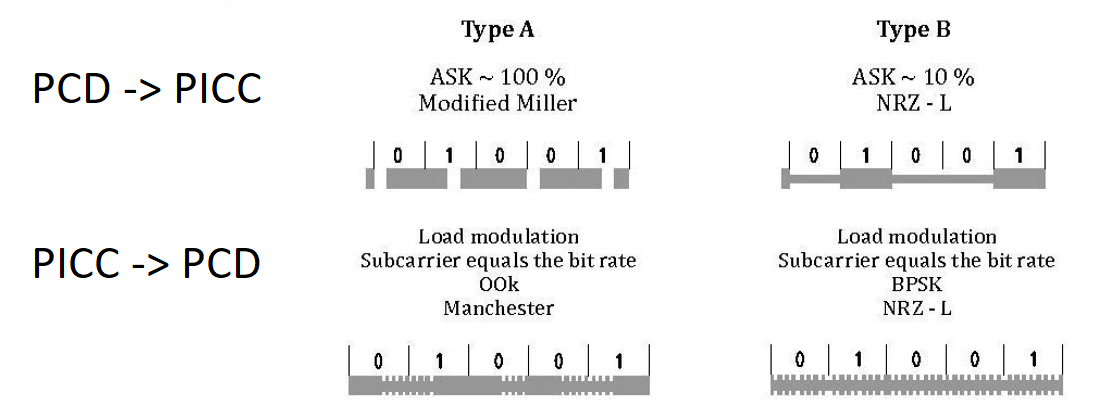
\includegraphics[scale=0.47]{./img/modulation_and_bit_encoding}
\caption{Comunicaciones con una tasa de bits de $\nicefrac{f_c}{128}$~\cite[Modificaciones Mías]{iso14443-2}}
\label{fig:mod-encode}
\end{figure}

Para PICCs de tipo A la modulación por comunicaciones desde el PCD hasta la PICC es ASK (Amplitude Shift Keying). Cuándo la amplitud de la portadora baja al 5\% del campo original, la norma define esto como una pausa. Un esquema de la misma se muestra en la \figref{fig:pause}, con valores que se definen en el \tabref{tab:pause_values}. Debido a que una PICC pasiva recibe su potencia inalámbricamente desde el campo electromagnético, es responsabilidad de la PICC mantener los rails de alimentación internos a tensiones adecuadas durante las pausas para que el sistema no cambie de estado. La codificación de los bits es Modified Miller. Cada trama comienza con un SOC (Start of Communication), tiene un número de bits de datos y termina con un EOC (End Of Communications). SOC, EOC y los valores lógicos son enviados mediante secuencias. Cada secuencia tiene el largo de una duración de bit, lo que es 128 ciclos de la portadora. La presencia y la ubicación de una pausa dentro de una duración de bit define el tipo de la secuencia, como es mostrado en la \figref{fig:sequences}. Una pausa que ocurre al principio de la duración de bit es una secuencia Z, una pausa que ocurre en el medio de la duración de bit es una secuencia X, y una bit sin pausas es una secuencia Y. El SOC es la secuencia Z. Un ‘1’ lógico es una X. Un ‘0’ lógico depende en la última secuencia, si fue una X, se envía una Y, si fue una Y o una Z, se envía una Z. La trama termina con el EOC lo que es un ‘0’ lógico, seguido por una secuencia Y. La \figref{fig:rx_frame_examples} muestra dos ejemplos de tramas.

\begin{figure}[htb]
  \centering
  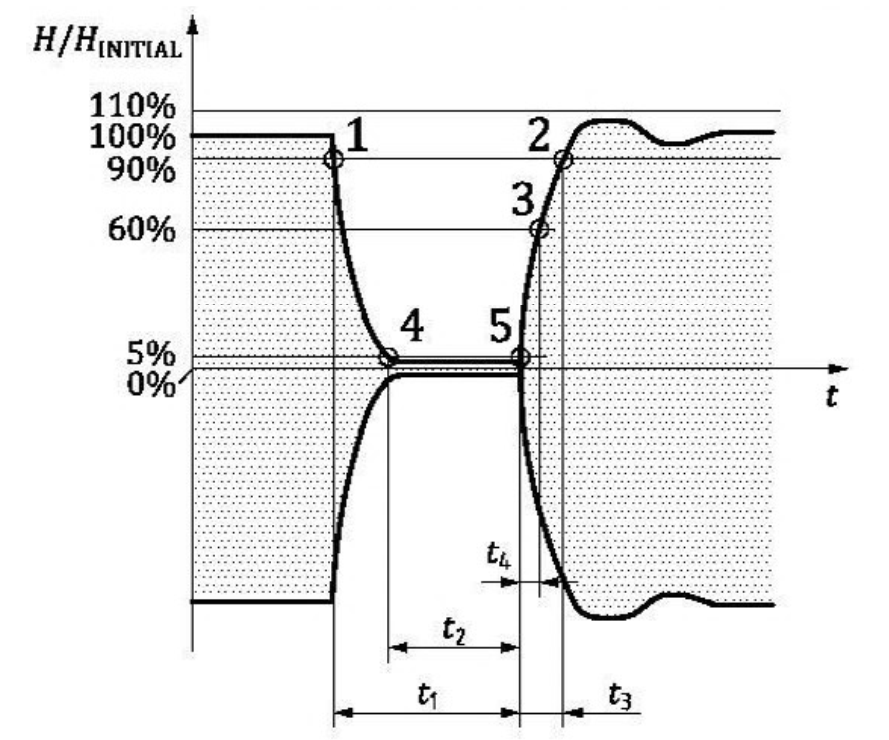
\includegraphics[scale=0.6]{./img/pause}
  \caption{El formato de una pausa tipo A~\cite{iso14443-2}}
  \label{fig:pause}
\end{figure}

\begin{table}[htb]
\centering
\begin{tabular}{|c|c|c|c|}
  \hline
  \textbf{Parámetro} & \textbf{Condición} & \textbf{Mínimo} & \textbf{Máximo} \\
  \hline
  $t_1$                   &                               & $\nicefrac{28}{f_c}$  & $\nicefrac{40,5}{f_c}$    \\
  \multirow{2}{*}{$t_2$}  & $t_1 > \nicefrac{34}{f_c}$  & $\nicefrac{7}{f_c}$   & \multirow{2}{*}{$t_1$}    \\
                          & $t_1 \le \nicefrac{34}{f_c}$  & $\nicefrac{10}{f_c}$  &                           \\
  $t_3$                   &                               & $1,5 \cdot t_4$           & $\nicefrac{16}{f_c}$      \\
  $t_4$                   &                               & 0                     & $\nicefrac{6}{f_c}$       \\
  \hline
\end{tabular}
\caption{Parámetros de timing para una pausa~\cite{iso14443-2}}
\label{tab:pause_values}
\end{table}

\begin{figure}[htb]
  \centering
  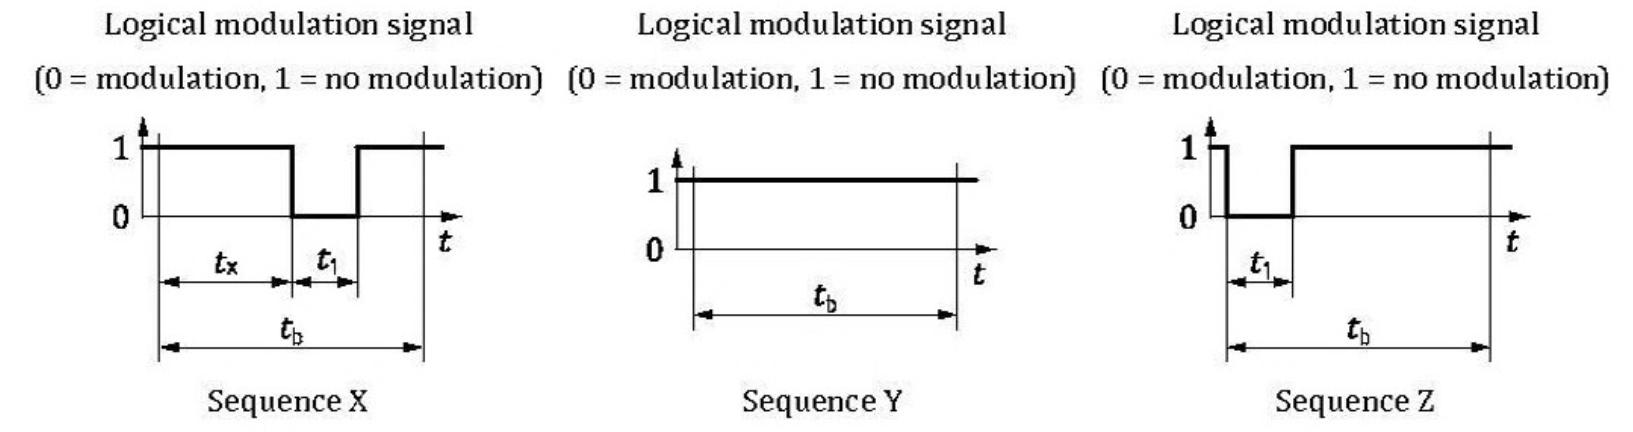
\includegraphics[scale=0.5]{./img/sequences}
  \caption{Codificación Modified Miller~\cite{iso14443-2}}
  \label{fig:sequences}
\end{figure}

\begin{figure}[htb]
  \centering
  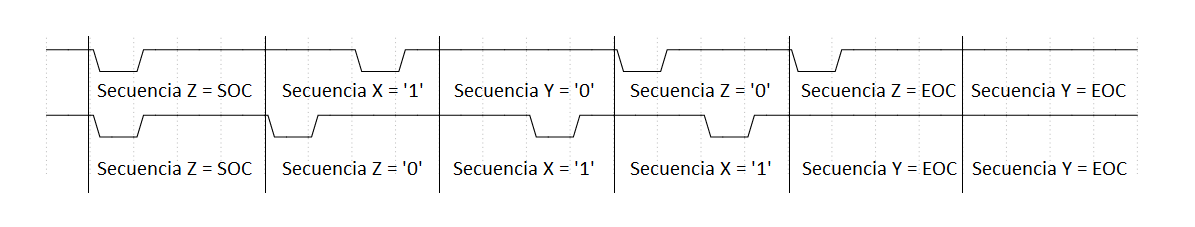
\includegraphics[scale=0.45]{./img/rx_frame_examples}
  \caption{Ejemplos de tramas PCD $\rightarrow$ PICC tipo A}
  \label{fig:rx_frame_examples}
\end{figure}

% There's a lot of images around here, make sure we keep them separated correctly
\FloatBarrier

Para responder las PICCs tipo A usan modulación de carga para generar una subportadora.  La frecuencia de la subportadora ($f_s$) depende de la tasa de bit. Para una tasa de bit de $\nicefrac{f_c}{128}$ la frecuencia es $\nicefrac{f_c}{16} \approx \SI{848}{\kilo\hertz}$. Como en el caso de comunicaciones del PCD a la PICC la duración de un bit es $\nicefrac{128}{f_c} = \nicefrac{8}{f_s}$. La portadora debe ser solo modulada con la subportadora cuando la PICC está enviando datos. Los bits a transmitir tienen codificación Manchester, para representar un ‘1’ lógico la señal es en ‘1’ por la primera mitad de la duración de bit, y en ‘0’ por la segunda mitad, para representar un ‘0’ lógico es al revés. La señal que maneja el modulador de carga es la operación lógica AND entre la señal de codificación Manchester y la subportadora como se muestra en la \figref{fig:picc_to_pcd}. Una trama comienza con un SOC lo que es un ‘1’ lógico, y termina con un EOC lo que es una duración de bit sin modulación, eso es a decir que la señal al modulador de carga es en ‘0’ por toda la duración de bit. La \figref{fig:tx_frame_example} muestra un ejemplo de una trama que ingresa a la compuerta AND con la subportadora.

\begin{figure}[htb]
  \centering
  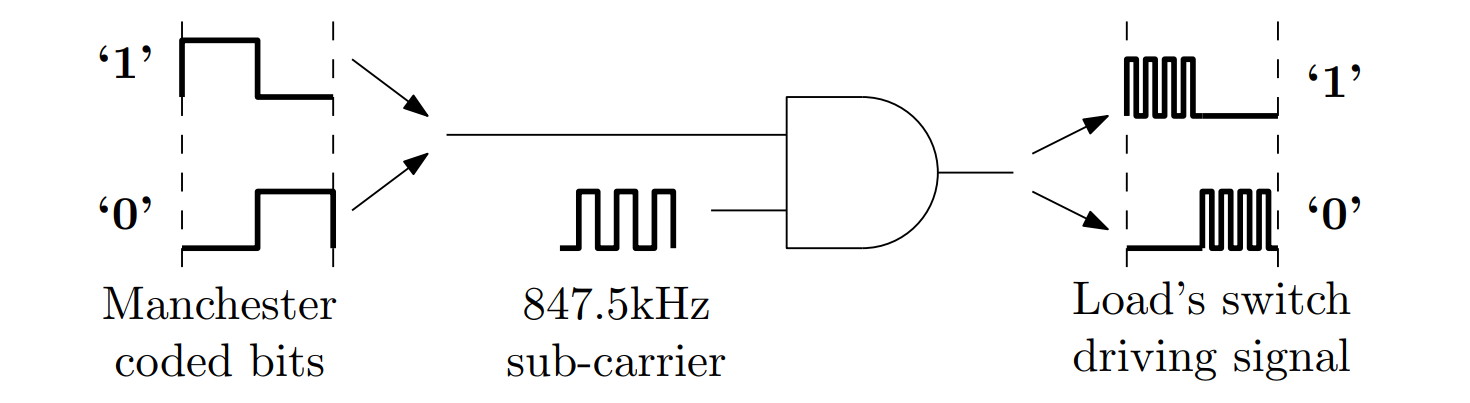
\includegraphics[scale=0.35]{./img/picc_to_pcd}
  \caption{Codificación de bits y modulación de la portadora con la subportadora para comunicaciones de la PICC a PCD~\cite{fabricio_eamta}}
  \label{fig:picc_to_pcd}
\end{figure}

\begin{figure}[htb]
  \centering
  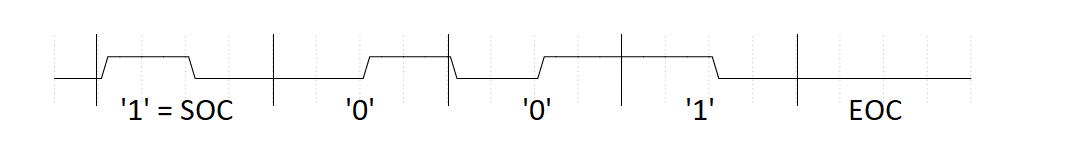
\includegraphics[scale=0.5]{./img/tx_frame_example}
  \caption{Ejemplo de una trama por comunicaciones PICC tipo A $\rightarrow$ PCD.}
  \label{fig:tx_frame_example}
\end{figure}

\FloatBarrier
\subsection{ISO/IEC 14443-3: \large{Inicialización y Anticolisión}}

La información presentada en esta sección es válida considerando una tasa de bit de fc/128 en cada dirección y PICCs tipo A.

La parte 3 de la norma define un FDT (Frame Delay Time), lo que es el tiempo entre dos tramas transmitidas en direcciones opuestas. Los tiempos del FDT definidos en la norma son especificados en números de ciclos de la portadora, y son medidos entre el último flanco de modulación de la primera trama y el primer flanco de modulación de la segunda trama. El \tabref{tab:fdt} muestra los FDTs especificados en la norma. En el caso del FDT entre una trama del PCD y una de la PICC, el FDT usado depende en el último bit lógico de la trama, y los valores especificados son absolutos para tramas de inicialización y tiempos mínimos para otras tramas.

\begin{table}[htb]
  \centering
  \begin{tabular}{|c|c|c|c|}
    \hline
    \textbf{Primera Trama} & \textbf{Segunda Trama} & \textbf{Último Bit} & \textbf{FDT} \\
    \hline
    \multirow{2}{*}{PCD~$\rightarrow$~PICC} & \multirow{2}{*}{PICC~$\rightarrow$~PCD} & '0' & 1172  \\
    \cline{3-4}
    & & '1' & 1236 \\
    \hline
    PICC~$\rightarrow$~PCD & PCD~$\rightarrow$~PICC & & 1272 \\
    \hline
  \end{tabular}
  \caption{Valores del FDT en número de ciclos de la portadora.}
  \label{tab:fdt}
\end{table}

Una trama comienza con un SOC, después se envían los datos empezando por el bit menos significativo, y termina con un EOC. Cada 8 bits de data hay un bit de paridad impar, así que el número de los 1s en cada byte más su bit de paridad es impar. Hay tres tipos de tramas definidas:

\begin{description}
  \item [Tramas Cortas] \hfill \\ Tienen siete bits de datos sin bit de paridad.
  \item[Tramas Estándares] \hfill \\ Tienen un número de bytes enteros, cada uno con un bit de paridad.
  \item[Tramas Anticolisión orientada a bits] \hfill \\ Tienen siete bytes cada uno con un bit de paridad, y están divididas en dos: la primera parte es enviada desde el PCD y la segunda parte desde la PICC. La partición puede ser después de un byte entero, incluyendo su bit de paridad (\figref{fig:anticollision} arriba), o en medio de un byte (\figref{fig:anticollision} abajo). Estas tramas son usadas durante el proceso de inicialización para que el PCD pueda detectar todas las PICCs en su campo electromagnético.
\end{description}

\begin{figure}[htb]
  \centering
  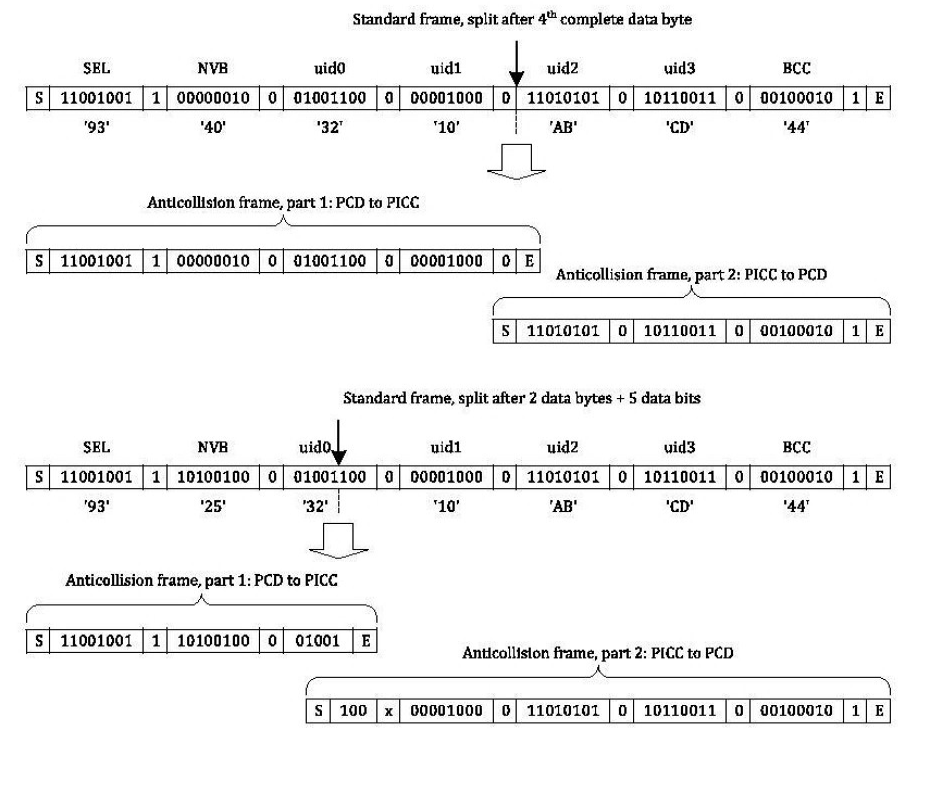
\includegraphics[scale=0.5]{./img/anticollision_frames}
  \caption{Trama Anticolisión orientada a bits~\cite[Modificaciones Mías]{iso14443-3}}
  \label{fig:anticollision}
\end{figure}

Unas de las tramas definidas en la norma terminan con un CRC16 (Cyclic Redundancy Check de 16 bits). El CRC16 permite el receptor de la trama determinar si el contenido fue corrompido. El polinomio del CRC es $P\left(x\right) = x^{16} + x^{12} + x^{5} + 1$, y el valor inicial es 0x6363~\cite{iso14443-3}\cite{iso13239}.

Cada PICC tiene un UID (Unique Identifier) que el PCD puede utilizar para enumerar todas las PICCs en su campo electromagnético y elegir cuáles activar. A pesar de que el nombre indique que el ID es único, no tiene que ser así. Está permitido usar un ID aleatorio (RID), o un ID no único (NUID). Los UIDs pueden ser: simples (4 bytes), dobles (7 bytes), o triples (10 bytes). Es requerido que todas las PICCs presentes en el campo de un PCD tienen UIDs únicos. Cuando se usan PICCs con NUIDs o RIDs es posible que haya conflictos. Debido a la gran cantidad de NUIDs posibles, la probabilidad de conflictos es mínima en un sistema bien diseñado.

Para identificar las PICCs presentes y activarlas, la norma define cinco comandos y sus respuestas, mostrados en el \tabref{tab:tramas}. La \figref{fig:14443-3-state-machine} especifica cómo una PICC debería responder cuando recibe un comando dependiendo de su estado actual.

\begin{table}[htb]
  \centering
  \begin{tabular}{l l l | l l l}
    \multicolumn{3}{c|}{\textbf{PCD $\rightarrow$ PICC}} & \multicolumn{3}{c}{\textbf{PICC $\rightarrow$ PCD}} \\
    \hline
    \textbf{Solicitud} & \textbf{Tipo} & \textbf{CRC} & \textbf{Respuesta} & \textbf{Tipo} & \textbf{CRC} \\
    \hline
    REQA & Corta & No & ATQA & Estándar & No \\
    WUPA & Corta & No & ATQA & Estándar & No \\
    ANTICOLLISION & Anticolisión & No & ANTICOLLISION & Anticolisión & No \\
    SELECT & Estándar & Sí & SAK & Estándar & Sí \\
    HLTA & Estándar & Sí & Sin Respuesta &  &  \\
  \end{tabular}
  \caption{Solicitudes y respuestas definidas en ISO/IEC 14443-3A}
  \label{tab:tramas}
\end{table}

\begin{figure}[htb]
  \centering
  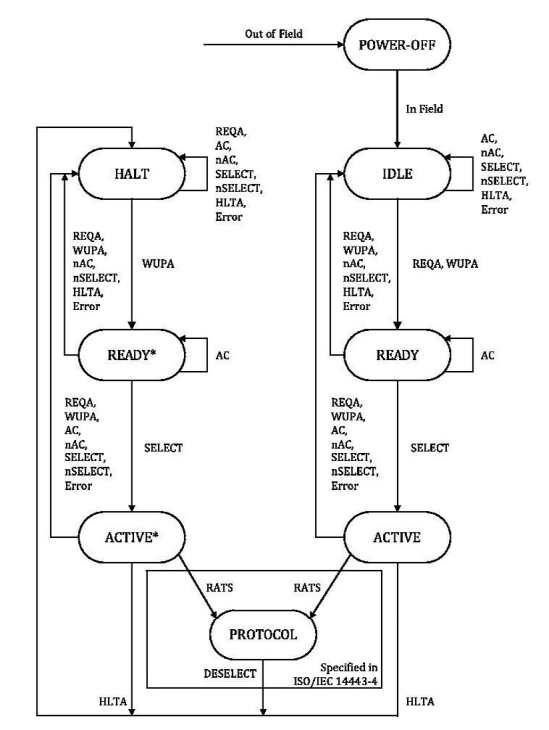
\includegraphics[scale=1]{./img/state_machine}
  \caption{Diagrama de transiciones de estados~\cite{iso14443-3}}
  \label{fig:14443-3-state-machine}
\end{figure}

\FloatBarrier

Cuando una PICC entra en un campo electromagnético, comienza en el estado IDLE. Un comando REQA o WUPA cambia el estado a READY. En ese estado el PCD puede enviar comandos de ANTICOLLISION para determinar el UID de una de las PICCs presentes. Con ese UID el PCD puede enviar un SELECT para mover la PICC al estado ACTIVE. Desde aquí el PCD puede enviar un RATS para terminar activando la PICC. En el caso de recibir un error, o un comando no esperado, la PICC vuelve al estado IDLE. Hay tres otros estados también: HALT, READY* y ACTIVE*. Las diferencias únicas entre estos estados y IDLE, READY y ACTIVE, son: WUPA es el único comando aceptado en HALT y el comando REQA es ignorado, y un error o un comando no esperado recibido en READY* o ACTIVE* causa la PICC volver a HALT en vez de IDLE. La ventaja de esto es que si el PCD decide que no quiere activar una PICC particular, puede ponerla en el estado HALT, y enviando un nuevo REQA comenzará el proceso de inicialización de nuevo en todos las PICCs menos aquellos que están en HALT.

En el caso de una PICC con UID doble el proceso de ANTICOLLISION y SELECT tiene que repetir dos veces antes de que la PICC se mueva al estado ACTIVE. En el primer lazo, los mensajes usan los primeros tres bytes de su UID junto con una etiqueta cascada: CT (Cascade Tag). La PICC responde al SELECT especificando que su UID no está completo todavía, y el lazo comienza de nuevo, esta vez usando los últimos cuatro bytes del UID. Por una PICC con UID triple este proceso tiene tres lazos. La \figref{fig:cascade_levels} muestra este proceso.

\begin{figure}[htb]
  \centering
  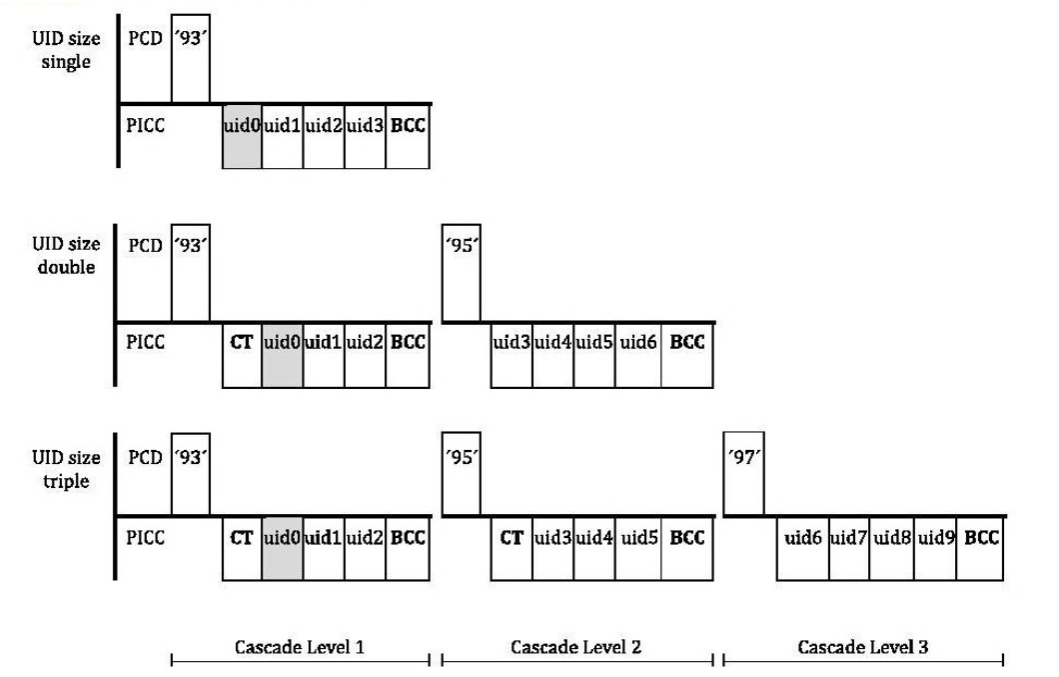
\includegraphics[scale=0.75]{./img/cascade_levels}
  \caption{Niveles cascadas para UIDs simples, dobles y triples~\cite{iso14443-3}}
  \label{fig:cascade_levels}
\end{figure}

El comando de ANTICOLLISION funciona de la siguiente forma: el PCD envía un UID parcial, y todas las PICCs en el campo electromagnético cuyas UIDs corresponden con la parte enviada, responden con los demás bits de sus UIDs. Debido al FDT fijo todas las PICCs comienzan responder de forma sincronizada. Las respuestas tienen codificación Manchester, por lo tanto cuándo dos PICCs envían valores lógicos diferentes el PCD puede detectar la colisión porque hay modulación durante todo el tiempo de bit. De esta manera el PCD sabe qué parte del UID es compartido entre todas las PICCs, y usando una búsqueda binaria puede determinar el UID completo de una de las PICC presentes. Esa PICC entonces puede ser activada o puesta en el estado HALT, y después el PCD puede repetir el proceso para enumerar todas las demás PICCs.

\FloatBarrier
\subsection{ISO/IEC 14443-4: \large{Protocolo de Transmisión}}

La mayor parte de esta subsección es común para PICCs tipo A y B, sin embargo hay dos comandos extras para terminar activando el protocolo para PICCs de tipo A. Estos comandos son RATS y PPS. El PCD debería enviar un RATS como el primer comando después de que una PICC entra en el estado ACTIVE o ACTIVE*. En el RATS el PCD asigna un CID (Card Identifier) a la PICC, esto es un identificador que el PCD puede usar para direccionar un mensaje a una PICC en particular, así que el CID debe ser único para cada PICC activa. En diferencia al UID, el CID solo tiene cuatro bits y son asignados  al momento de la inicialización y no en la  de fabricación. Este CID es válido sólo hasta que la PICC es desactivada. La respuesta al RATS es la ATS lo que contiene información sobre la capacidad de la PICC, por ejemplo las tasas de bits y el tamaño máximo de una trama que la PICC puede recibir. El comando PPS es opcional, y solo puede ser enviado inmediatamente después de que el PCD recibe la ATS. El PPS permite al PCD configurar las tasas de bits de comunicaciones en cada dirección.

La norma define dos formatos de bloques: estándares y aumentados. Bloques estándares están enviados en tramas estándares con el CRC16 presente. Bloques aumentados comienzan con el largo del bloque, y terminan con un CRC32, y el campo INF contiene códigos Hammings para la corrección de errores. La \figref{fig:std_enhanced_blocks} muestra los dos. Comunicaciones comienza con bloques estándares hasta que el PCD configura lo contrario.

\begin{figure}[htb]
  \centering
  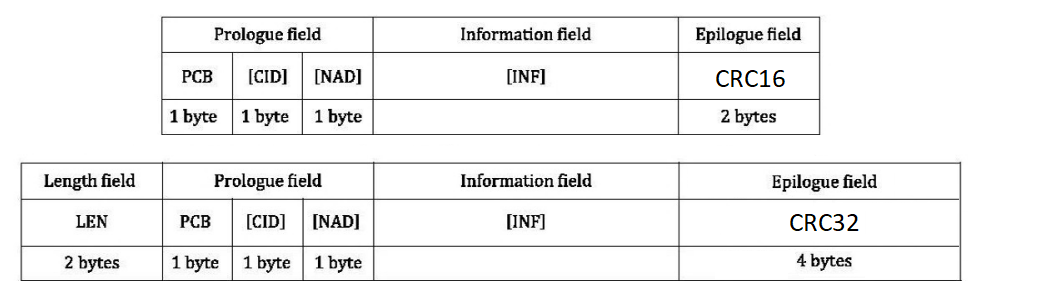
\includegraphics[scale=0.52]{./img/bloque_formats}
  \caption{El formato de un bloque estándar (arriba) y uno aumentado (abajo)~\cite{iso14443-4}}
  \label{fig:std_enhanced_blocks}
\end{figure}

Hay tres tipos de bloques: I (Information), R (Receive Ready) y S (Supervisory). El campo PCB indica que tipo de bloque es. El CID es la dirección de la PICC y solo está presente si la PICC lo soporta. El campo CID en respuestas también contiene dos bits con información sobre el nivel de potencia recibido, el PCD puede usar esa información para controlar la potencia transmitida por el campo. La NAD (Node Address) permite una PICC tener más de una aplicación, direccionado por este campo, también solo está presente si la PICC la soporta. Finalmente el campo INF contiene la información del bloque, y solo es presente por bloques tipos I y S.

Bloques-S son usados para información de control. Hay tres comandos definidos:

\begin{description}
  \item[S(WTX)] \hfill \\ Waiting Time eXtension. Si la PICC no está lista para responder a una solicitud en el tiempo permitido, puede responder con un S(WTX) pidiendo más tiempo.
  \item[S(DESELCT)] \hfill \\ Este comando es enviado por el PCD cuándo quiere desactivar la PICC.
  \item[S(PARAMETERS)] \hfill \\ Este comando está usado para leer o setear la configuración de la PICC. Por ejemplo, para cambiar la tasa de bits, o cambiar entre bloques estándares y aumentados.
\end{description}

Bloques-I son usados para transmitir información al nivel de aplicación. El protocolo de la aplicación no está definido en esta norma. Estos bloques pueden ser encadenados para permitir el envío de un mensaje más grande que el soportado por el destino, partiendo el mensaje en partes de tamaños soportados.

Bloques-R son usados para reconocer la recepción de un bloque: R(ACK) o indicar errores: R(NAK). En el caso de bloques-I encadenados un R(ACK) es enviado para pedir la siguiente parte del mensaje. También el PCD puede enviar un R(ACK/NAK) para pedir la PICC retransmita su última respuesta, esto puede ser usado para recuperar de errores. Finalmente el PCD puede enviar un R(NAK) para verificar la presencia continua de la PICC.

% ---------------------------------------------
% Descripción General del Proyecto Marco
% ---------------------------------------------

\FloatBarrier
\chapter{Descripción General del Proyecto Marco}

Este trabajo se enmarca en un proyecto que tiene como objetivo general desarrollar un circuito integrado capaz de tomar muestras de un sensor MOSFET de radiación y transmitirlas a un dispositivo externo mediante un protocolo propietario implementado encima de la norma ISO/IEC 14443A. Este proyecto marco requiere cinco bloques como se muestra en la \figref{fig:entire_project}:

\begin{figure}[htb]
  \centering
  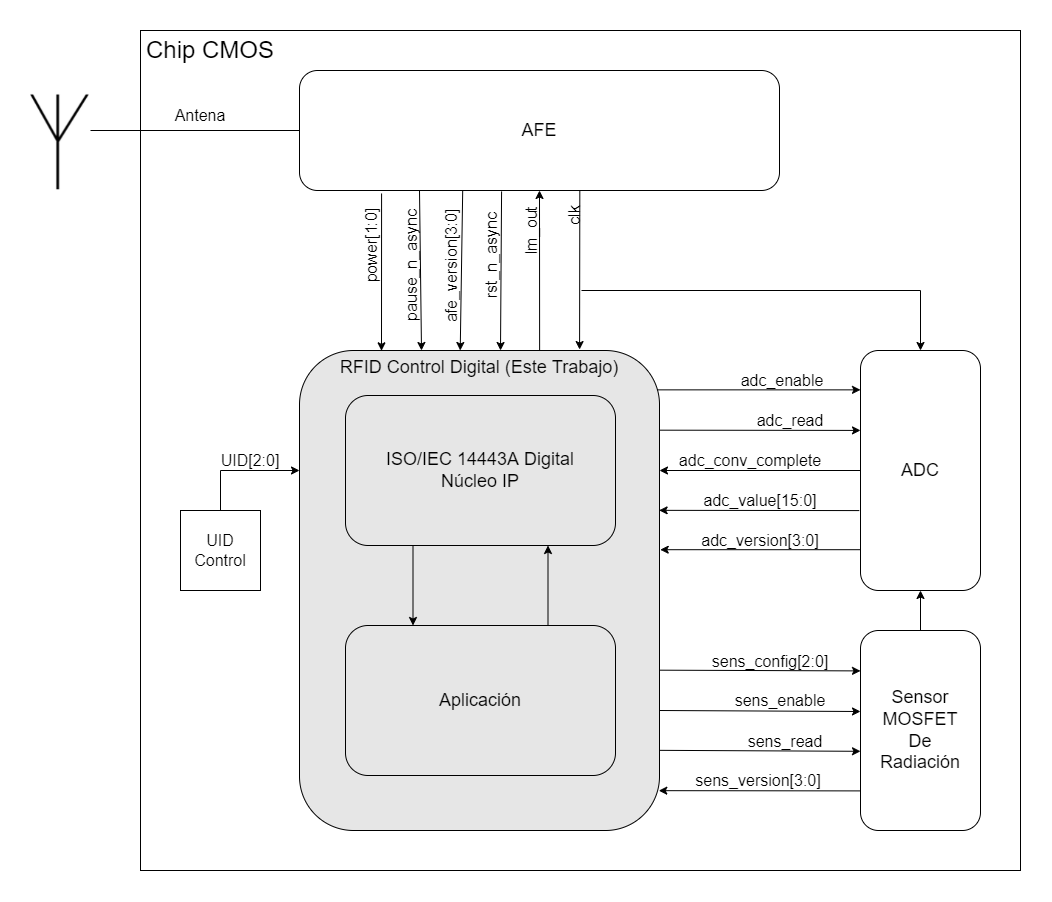
\includegraphics[width=0.95\textwidth]{./img/entire_project_v2}
  \caption{Diagrama general del proyecto marco y su relación con el bloque a diseñar en esta Tesis.}
  \label{fig:entire_project}
\end{figure}

\begin{description}
  \item[El Analogue Front End (AFE)] \hfill \\ Es la parte analógica de la norma ISO/IEC 14443A-2.
  \item[El sensor MOSFET de radiación] \hfill \\ Desarrollado por el Laboratorio de Física de Dispositivos-Microelectrónica (LFDM) de la facultad de ingeniería de la UBA.
  \item[El Conversor Analógico Digital (ADC, por sus siglas en inglés)] \hfill \\ Encargado de convertir la salida analógica del sensor a una señal digital.
  \item[El RFID Control Digital] \hfill \\ Es el objetivo de esta Tesis.
  \item[El UID Control] \hfill \\ Permite asignar la parte variable del UID de la PICC.
\end{description}

Algunos de estos bloques no se han desarrollado todavía, por lo que es necesario asumir las especificaciones de los mismos.

El AFE es responsable de:

\begin{itemize}
  \item Recibir y regular potencia desde el campo electromagnético. La implementación de esta tesis se realiza considerando la tecnología de fabricación de XFAB 180 nm, la cual utiliza celdas estándares que requieren una tensión de 1.8 V, por lo que el AFE debe producir esa tensión, y mantenerla durante las pausas.
  \item Recuperar la señal de reloj a partir de la portadora. La dificultad en este punto reside en el hecho de que el PCD envía información a la PICC utilizando pausas en la portadora, por lo cual se espera que el reloj se detenga durante estas pausas. Es posible utilizar un PLL para producir un reloj continuo. El circuito de esta tesis es elaborado con habilidad para funcionar con un reloj continuo o con un reloj que se detenga durante las pausas. En la \secref{sec:sequence_decode}{sequence\_decode} se detalla el número máximo de flancos del reloj que es posible perder conservando una correcta decodificación de las secuencias.
  \item Manejar la señal de reset (activa baja). Los demás bloques se deben mantener en un estado de reset hasta que la tensión de alimentación sea estable.
  \item Detectar las pausas enviadas desde el PCD.
  \item Permitir la transmisión de respuestas al PCD mediante un modulador de carga. El modulador debería ser manejado directamente desde una entrada del bloque, lo cual sería conectado a la salida \textit{lm\_out} del bloque RFID Digital Control. La señal se obtiene como el AND lógico de la codificación Manchester y la subportadora.
  \item Generar una señal indicando el nivel de potencia recibida a través del campo electromagnético (opcional). Si se tiene esta información, la misma puede ser enviada al PCD en el campo CID de mensajes de nivel protocolo. El PCD puede usarla para ajustar la intensidad del campo electromagnético.
  \item Proveer una salida de cuatro bits que indique la versión del hardware del AFE. Este valor forma parte de la información enviada al PCD como respuesta al mensaje de protocolo IDENTIFY.
\end{itemize}

El sensor de radiación tiene tres entradas: \textit{sens\_config[2:0]}, \textit{sens\_enable} y \textit{sens\_read} . Para leer el sensor, primero se debe establecer el valor de \textit{sens\_config[2:0]} de manera que se elija la configuración del sensor deseado por el usuario. Posteriormente se debe establecer \textit{sens\_enable} en ‘1’ para activar el sensor. Finalmente después del tiempo deseado por el usuario, llevar \textit{sens\_read} a ‘1’ configura al circuito del sensor en modo lectura para su muestreo. Por otro lado, el sensor tiene dos salidas, una analógica que está conectada al ADC, y una señal de cuatro bits que indica la versión del sensor. Este valor forma parte de la información enviada al PCD como respuesta al mensaje de protocolo IDENTIFY.

Por su parte el ADC, además de la entrada analógica proveniente desde el sensor, tiene otras dos entradas: \textit{adc\_enable} y \textit{adc\_read}. El flanco ascendente de la señal \textit{adc\_read} indica el momento de muestreo de la salida del sensor.. Respecto de las salidas, hay tres: \textit{adc\_conversion\_complete}, \textit{adc\_value[15:0]} y \textit{adc\_versión[3:0]}. Cuando el ADC completa la conversión la señal \textit{adc\_conversion\_complete} toma el valor '1' durante un ciclo del reloj. La señal \textit{adc\_value} debe ser estable antes del pulso en \textit{adc\_conversion\_complete}.

El bloque de UID Control es responsable de especificar los tres bits más bajos del UID de la PICC. Este valor puede ser configurado mediante una memoria no volátil, pero en esta tesis la intención es configurarlo utilizando wire bonding o resistores pull up/down.

El objetivo de esta tesis es implementar el bloque del RFID Control Digital, que consiste en dos sub-bloques: Una implementación del parte digital de la norma ISO/IEC 14443A y un protocolo a nivel aplicación que permita la lectura del sensor y envíe esta información al PCD. Un requisito de este bloque es que la entrada de UID se mantenga estable mientras el bloque no esté en un estado de reset.

% --------------------------------------------
% Implementación y Verificación
% ---------------------------------------------

\FloatBarrier
\chapter{Implementación y Verificación}

La implementación de todos los módulos y los bancos de prueba se escriben con el HDL (Hardware Description Language) SystemVerilog, el cual  es definido en IEEE 1800~\cite{ieee1800}. SystemVerilog es basado en Verilog,  formalmente definido en IEEE 1364~\cite{ieee1364}. SystemVerilog es conocido principalmente como un HDL para verificación debido a sus extensiones sustanciales a verilog en ese ámbito, por ejemplo en la adicción de conceptos de programación orientados a objetivos (como clases), y aserciones. Además SystemVerilog tiene varias ventajas a Verilog para uso en síntesis~\cite{synthesisable_sv}, por ejemplo:

\begin{description}
  \item[Enumeraciones (enum) y estructuras (struct)] \hfill \\ Como en el lenguaje de programación C.
  \item[always\_comb y always\_ff] \hfill \\ Estos permiten al ingeniero especificar su intención a implementar lógica combinatoria o secuencial respectivamente. Las herramientas pueden verificar que el circuito inferido cumple con esa intención, por ejemplo, que los bloques combinatorios no contienen latches.
  \item[Interfaces] \hfill \\ Colecciones de señales que son frecuentemente usadas juntas para reducir la replicación de código.
\end{description}

La implementación de esta tesis está dividida en dos: 1) El núcleo IP genérico para ISO/IEC 14443A que es la lógica digital necesaria para recibir, decodificar y actuar sobre los mensajes definidos en la norma, y construir, codificar y transmitir las respuestas adecuadas. Este núcleo IP está dividido en tres partes principales, uno para cada parte de la norma (excepto ISO/IEC 14443-1). 2) El sistema de control del sensor y del ADC. La \figref{fig:top_level} muestra todos esos bloques, y el flujo de datos entre ellos.

\begin{figure}[htb]
  \centering
  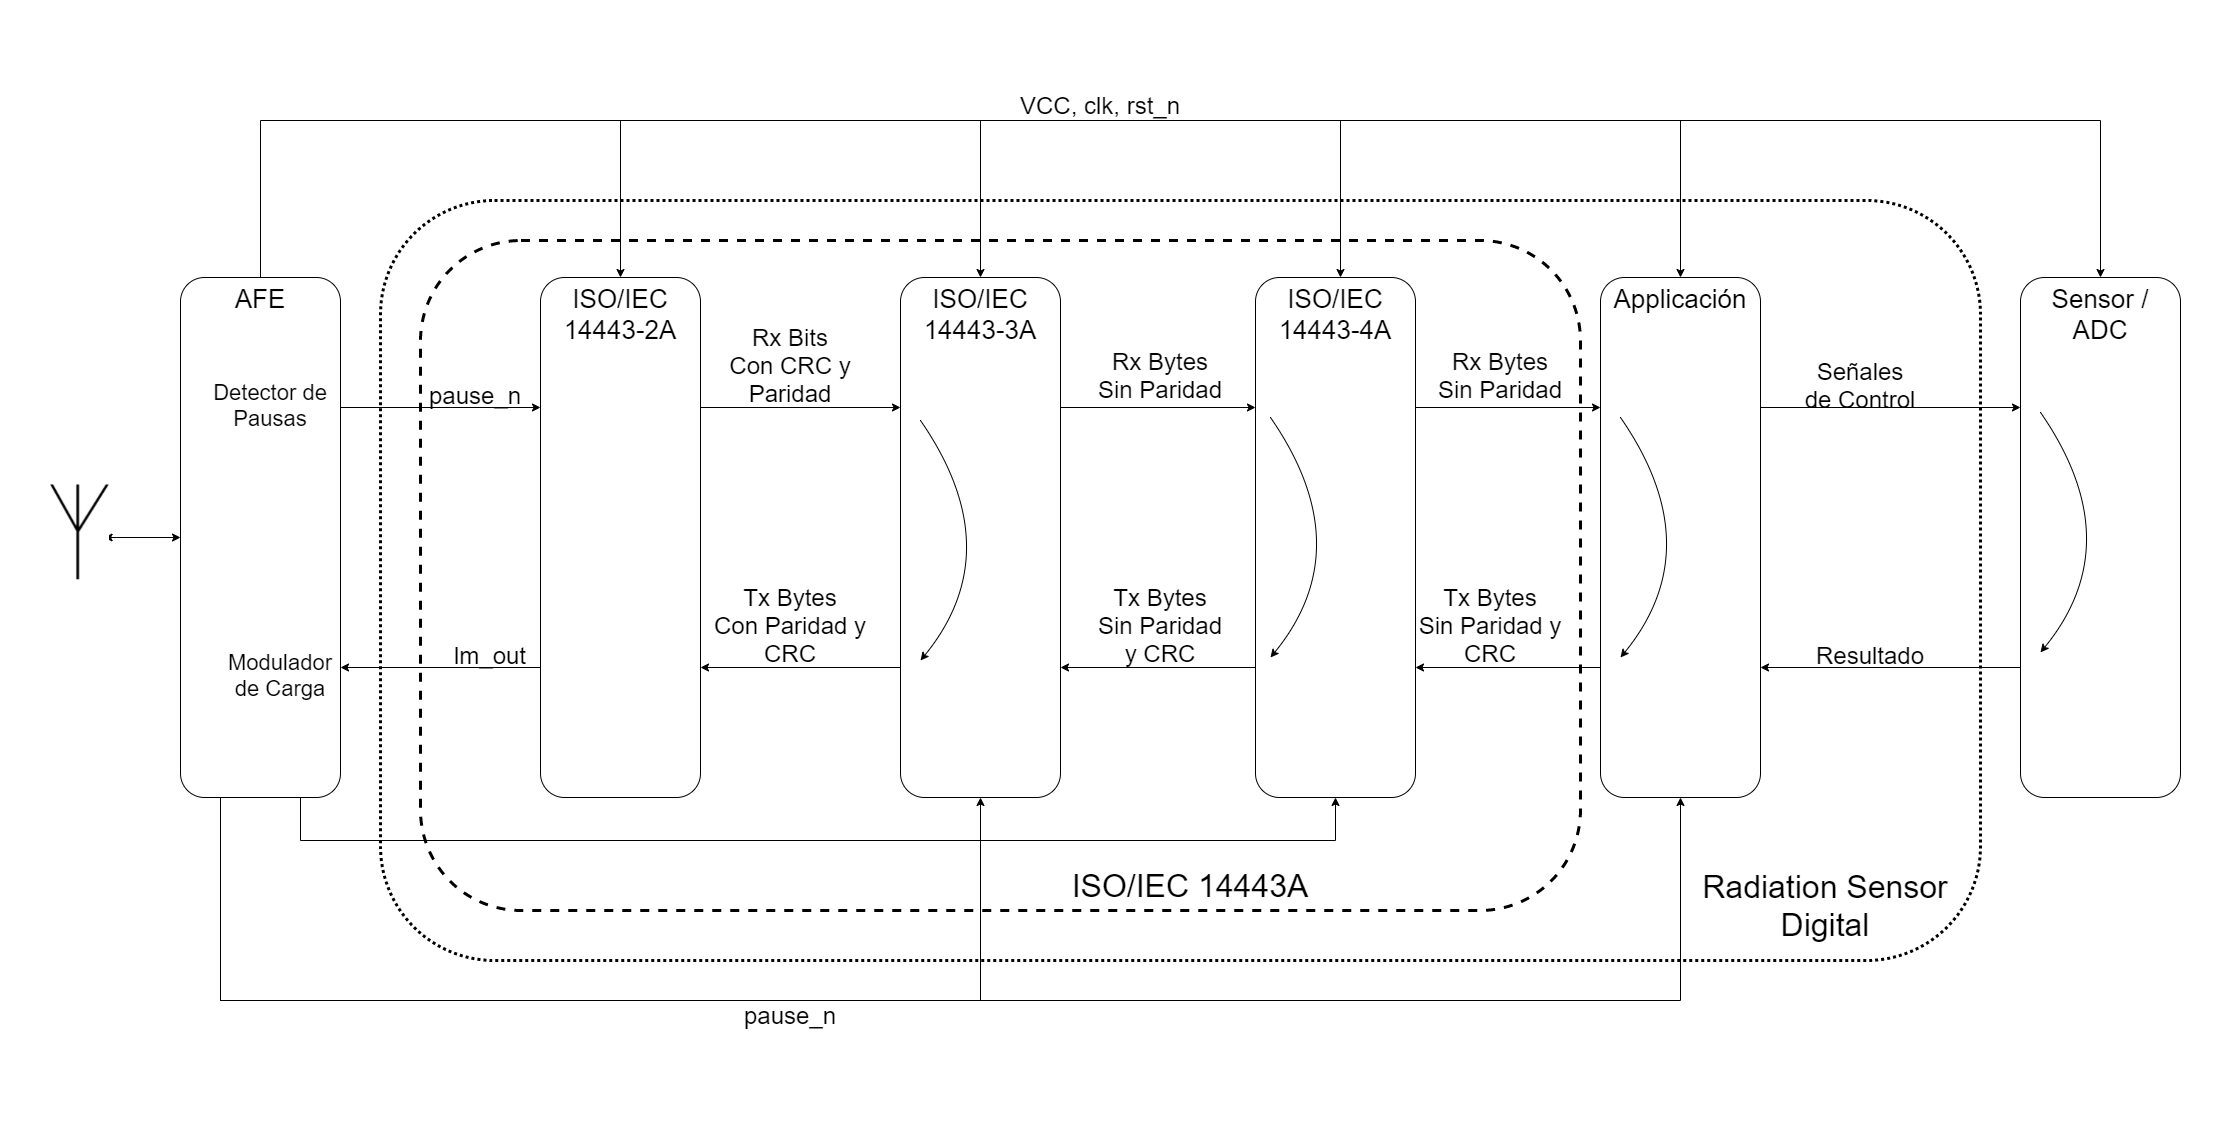
\includegraphics[width=1.0\textwidth]{./img/top_level}
  \caption{Los bloques principales de la implementación.}
  \label{fig:top_level}
\end{figure}

% Interfaces
% --------------------------------
\FloatBarrier
\section{Interfaces}

La norma IEEE de SystemVerilog define un interfaz como:

\begin{displaycquote}[traducción mía]{ieee1800}
A su nivel más bajo, un interfaz es un conjunto nombrado de nets o variables. La interfaz es instanciada en un diseño y puede ser accedida por un puerto como un ítem sencillo; las nets o variables componentes [pueden ser] referidos cuando sea necesario. Una proporción significativa de un diseño verilog frecuentemente consiste en listas de puertos y listas de conexiones, los que son simplemente repeticiones de nombres. La habilidad de reemplazar un grupo de nombres con un nombre simple puede reducir significativamente el tamaño de una descripción y mejorar su mantenibilidad. 
\end{displaycquote}

Además de esas ventajas, una interfaz puede contener funcionalidad, sea para síntesis o verificación, por ejemplo se puede agregar aserciones que verifican el comportamiento de los nets internos en vez de tener que duplicar esas pruebas en cada sitio que la interfaz es usada. Una interfaz puede tener una o más modports, los que especifican las direcciones de las señales. Esos modports pueden ser usados en la lista de puertas por un módulo en vez de especificar cada señal y su dirección individualmente.

Este trabajo consiste en varios módulos que contienen uno o más sumideros para recibir tramas desde otros módulos, y una o más fuentes para enviar tramas a otros módulos. Por ejemplo el módulo: \textbf{frame\_decode} recibe tramas desde el módulo: 

La \textit{rx\_interface} contiene:

\begin{itemize}
  \item \textit{soc}: Un indicador que indica el comienzo de una trama.
  \item \textit{eoc}: Un indicador que indica el fin de una trama.
  \item \textit{data}: Un bit / byte de la trama.
  \item \textit{data\_valid}: Un indicador que indica si los datos en \textit{data} son válidos.
  \item \textit{data\_bits}: La cantidad de bits válidos. Por una interfaz configurada a bytes, esta señal permite la recepción de tramas cortas que tienen solo 7 bits, o de tramas anticolisión orientada a bits que pueden terminar con entre uno y ocho bits.
  \item \textit{error}: Indica la detección de un error en la trama, por ejemplo: un bit de paridad equivocado.
\end{itemize}


La \figref{fig:rx_iface} muestra una simulación de la recepción de una trama corta con una \textit{rx\_interface} de bits, y su conversión a una serie de bytes. Arriba están las señales en una \textit{rx\_interface} de bits, \textit{data\_valid} está en ‘1’ siete veces durante la trama, indicando que el dato recibido es: 1,1,1,1,0,1,0. Debido a que el bit menos significativo es enviado primero, este serie representa 7’b0101111. Abajo están las señales en una \textit{rx\_interface} de bytes representando la misma trama. El dato tiene valor 7’b0101111 cuando \textit{data\_valid} tiene valor lógico igual a ‘1’.

La \textit{rx\_interface} incluye varias aserciones para verificar el comportamiento de las señales en la interfaz. Las aserciones consideran: Las señales son correctas en el estado de reset, los indicadores nunca son desconocidos, \textit{soc} y \textit{eoc} no están en ‘1’ en el mismo ciclo, y que solo están en ‘1’ por la duración de un solo ciclo del reloj a la vez.

\begin{figure}[htb]
  \centering
  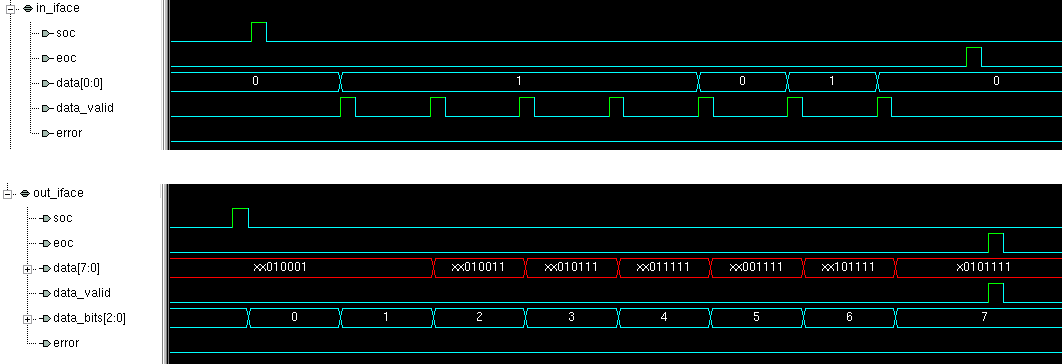
\includegraphics[width=1.0\textwidth]{./img/rx_iface_example}
  \caption{Una simulación de la recepción de una trama corta representada con una \textit{rx\_interface} de bits (arriba) y su conversión a una \textit{rx\_interface} de bytes (abajo).}
  \label{fig:rx_iface}
\end{figure}

\FloatBarrier

La \textit{tx\_interface} contiene:

\begin{itemize}
  \item \textit{data}: Un bit / byte de la trama.
  \item \textit{data\_valid}: Un indicador que indica que \textit{data} es válida.
  \item \textit{data\_bits}: La cantidad de bits válidos. Para una interfaz configurada a bytes, esta señal permite la transmisión de tramas de anticolisión orientada a bits, las que pueden comenzar con un byte parcial.
  \item \textit{last\_bit\_in\_byte}: Esta señal solo existe en interfaces de bits. Indica que el bit actual es el último bit en un byte. Es usado para conocer dónde agregar bits de paridad dentro de una serie de bits.
  \item \textit{req}: El sumidero usa esta señal para pedir que la fuente envíe el siguiente bit / byte de la trama. La norma ISO/IEC 14443A-2 define la duración de bits como 128 ciclos de la portadora, por lo tanto esta señal es necesaria para limitar la tasa de envío de datos.
\end{itemize}

Cuándo una fuente está lista para transmitir una trama se establece el primer bit / byte de la trama en la señal \textit{data} y fija \textit{data\_valid} en ‘1’. El sumidero puede utilizar la señal \textit{data\_valid} para ver si la fuente tiene data enviar. Después de haber leído la primera bit / byte de data, el sumidero fija la señal \textit{req} en ‘1’ durante un ciclo del reloj. La fuente detecta ese pulso y si hay más data a enviar, se actualiza la \textit{data} con el siguiente bit / byte, dejando \textit{data\_valid} en ‘1’. Este proceso repite hasta que la fuente no tiene más data a enviar, y después del último pulso en la \textit{req}, se fija \textit{data\_valid} en ‘0’. La \figref{fig:tx_iface} muestra una simulación de la transmisión de una trama de 16 bits con una \textit{tx\_interface} de bytes, y su conversión a una serie de bits. Arriba están las señales en la \textit{tx\_interface} de bytes enviando la data 0xAE, 0x42. Abajo están las señales en una \textit{tx\_interface} de bits representando la misma trama.

La \textit{tx\_interface} también incluye tres aserciones que verifican: Las señales son correctas en el estado de reset, \textit{req} es ‘1’ solo para la duración de un ciclo del reloj, y que \textit{data}, \textit{data\_valid}, \textit{data\_bits} y \textit{last\_bit\_in\_byte} solo cambian estado cuando \textit{data\_valid} está ‘0’ o en los cuatro ciclos después de un pulso de req. La última aserción es para verificar que la fuente puede proveer datos cuándo es pedido con la señal \textit{req} antes de que el sumidero la necesita.

\begin{figure}[htb]
  \centering
  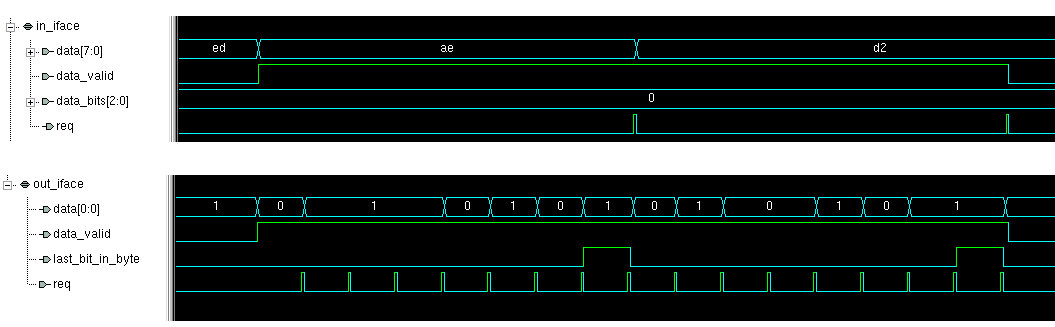
\includegraphics[width=1.0\textwidth]{./img/tx_iface_example}
  \caption{Una simulación de la transmisión de una trama de 16 bits representada con una \textit{tx\_interface} de bytes (arriba) y su conversión a una \textit{tx\_interface} de bits (abajo).}
  \label{fig:tx_iface}
\end{figure}


% Marco de Verificación
% --------------------------------
\FloatBarrier
\section{Marco de Verificación}

Simulación y verificación es una parte muy importante del diseño digital. En un informe de 2020 sobre las tendencias de diseño y verificación de ICs y ASICs~\cite{verification_trends_2020}, los autores encontraron que en promedio más de 50\% del tiempo de un proyecto es utilizado en verificación. También encontraron que en promedio hay un ingeniero de verificación por cada ingeniero de diseño, además los ingenieros de diseño gastan aproximadamente la mitad de su tiempo verificando sus diseños.

En esta tesis se utiliza verificación funcional mediante simulaciones con la herramienta VCS de Synopsys. Las simulaciones son completamente automatizadas y son ejecutadas con un comando sencillo utilizando un Makefile, por ejemplo: “make serialiser\_tb”.

UVM (Universal Verification Methodology) es una metodología de verificación funcional mediante un conjunto de clases de SystemVerilog. Casi 80\% de proyectos mundiales son verificados con UVM~\cite{verification_trends_2020}. Una de las ventajas principales de UVM es la modularidad. El código es partido en bloques separados facilitando la reutilización de los componentes en varios bancos de pruebas sin tener que duplicar código. La desventaja principal es la complejidad, requiere mucho código para armar un banco de prueba. UVM no es usada en esta tesis porque su implementación sería más compleja que el propio diseño. Sin embargo el marco de verificación está basado en las técnicas de UVM.

El proceso de verificación es estimular las entradas del DUT (Design Under Test) y verificar que las salidas son las esperadas. Frecuentemente no es posible verificar un diseño para todas las combinaciones y secuencias posibles de las entradas, por lo tanto es común usar estímulo aleatorio. Con estímulo aleatorio siempre hay el riesgo de no verificar parte del diseño, por la posibilidad de no elegir una de las combinaciones o secuencias de entradas necesarias para estimular esa parte del diseño. Una técnica para ayudar a mitigar esto, es: aleatorio restringido (constrained random), esta técnica permite la generación de estímulo aleatorio mediante constraints para restringir el estímulo a un rango interesante en particular. Por ejemplo, en vez de generar tramas completamente aleatorias, pueden ser limitadas: a tramas válidas, una colección de tramas en particular, o tramas con errores.

Una técnica para asegurar que todas las partes de un diseño son verificadas suficientemente, es generar informes de cobertura. La herramienta VCS está habilitada para generar, de forma automática, informes de cobertura de código con varias métricas, y un resultado total de qué proporción del diseño fue verificado. Estos informes pueden ser analizados por el diseñador para verificar cuáles partes de su diseño fue suficientemente estimulado y cuáles partes necesitan más trabajo. Las métricas de cobertura de código habilitadas en VCS son:

\begin{itemize}
  \item Línea: Muestra las líneas del RTL que fueron ejecutadas.
  \item Condición: Muestra las sub expresiones booleanas que fueron evaluados a verdadero y falso. Por ejemplo en la declaración: “res = (A == 0) ? B : C”, el informe de cobertura indicará si la expresión “A == 0” fue evaluado al menos una vez a verdadero y al menos una vez a falso.
  \item Cambio de Estado (Toggle): Muestra cuáles señales y puertas cambiaron de estado en las dos direcciones.
  \item Branch: Muestra cuáles branches fueron tomados.
  \item FSM (Finite State Machine): Muestra cuáles estados en un FSM fueron utilizados, y las transiciones entre ellos.
  \item Aserción: Muestra cuáles aserciones fueron: ejecutadas, aprobadas y falladas, y cuántas veces por cada uno.
\end{itemize}

El marco de verificación es implementado con varios componentes, la mayoría son clases de SystemVerilog. Los componentes pueden ser divididos en siete grupos distintos:

\begin{itemize}
  \item Transacciones: Una transacción representa una trama, puede ser una trama de bits, de bytes o de secuencias (como definido en ISO/IEC 14443-2).
  \item Controladores: Un controlador envía una transacción sobre una interfaz.
  \item Monitores: Un monitor monitoriza una interfaz, y construye transacciones representando las tramas detectadas.
  \item Generador de transacciones: Genera transacciones de bytes para representar las tramas definidas en la norma. También puede generar transacciones aleatoriamente.
  \item Convertidor de transacciones: Produce una transacción en un formato desde una transacción en otro formato. Por ejemplo puede convertir una transacción de bytes a una transacción de bits, opcionalmente agregando los bits de paridad.
  \item Secuencias: Código compartido para verificar diseños que reciben tramas, actúan sobre ellos, y generan las respuestas. Por ejemplo: cuándo el DUT está en el estado READY, responde a un SELECT con un SAK con los valores esperados, y se transiciona al estado ACTIVE. Ese ejemplo es una prueba utilizada para verificar el comportamiento de cuatro módulos: \textbf{initialization}, \textbf{iso14443\_3a}, \textbf{iso14443a}, \textbf{radiation\_sensor\_digital\_top}.
  \item Otros: Este grupo incluye: modelos de los bloques analógicos, una clase para guardar la dirección de una PICC (UID, CID y NAD), y unas interfaces que solo están usadas para verificación.
\end{itemize}

% Transacciones
\FloatBarrier
\subsection{Transacciones}

% Controladores
\FloatBarrier
\subsection{Controladores}

% Monitores
\FloatBarrier
\subsection{Monitores}

% Generador y Conversores de Transacciones
\FloatBarrier
\subsection{Generador y Conversores de Transacciones}

% Secuencias
\FloatBarrier
\subsection{Secuencias}

% Otros
\FloatBarrier
\subsection{Otros}

% Modelos Analógicos
\FloatBarrier
\subsubsection{Modelos Analógicos}

% Estructura de los Bancos de Pruebas
\FloatBarrier
\subsection{Estructura de los Bancos de Pruebas}

% ISO/IEC 14443A núcleo IP
% --------------------------------
\FloatBarrier
\section{ISO/IEC 14443A núcleo IP}

% ISO/IEC 14443-2A
\FloatBarrier
\subsection{ISO/IEC 14443-2A}

% subcarrier
\FloatBarrier
\subsubsection{subcarrier}

% bit_encoder
\FloatBarrier
\subsubsection{bit\_encoder}

% tx
\FloatBarrier
\subsubsection{tx}

% sequence_decode
\FloatBarrier
\subsubsection{sequence\_decode}
\label{sec:sequence_decode}

% iso14443_2a
\FloatBarrier
\subsubsection{iso14443\_2a}

% ISO/IEC 14443-3A
\FloatBarrier
\subsection{ISO/IEC 14443-3A}

% frame_decode
\FloatBarrier
\subsubsection{frame\_decode}

% deserialiser
\FloatBarrier
\subsubsection{deserialiser}

% FDT
\FloatBarrier
\subsubsection{FDT}

% CRC_A
\FloatBarrier
\subsubsection{CRC\_A}

% crc_control
\FloatBarrier
\subsubsection{crc\_control}

% serialiser
\FloatBarrier
\subsubsection{serialiser}

% frame_encode
\FloatBarrier
\subsubsection{frame\_encode}

% framing
\FloatBarrier
\subsubsection{framing}

% routing
\FloatBarrier
\subsubsection{routing}

% initialisation
\FloatBarrier
\subsubsection{initialisation}

% ISO/IEC 14443-3A
\FloatBarrier
\subsubsection{ISO/IEC 14443-3A}

% ISO/IEC 14443-4A
\FloatBarrier
\subsection{ISO/IEC 14443-4A}

% ISO/IEC 14443A
\FloatBarrier
\subsection{ISO/IEC 14443A}

% Otros
\FloatBarrier
\subsection{Otros}

% synchroniser
\FloatBarrier
\subsubsection{synchroniser}

% active_low_reset_synchroniser
\FloatBarrier
\subsubsection{active\_low\_reset\_synchroniser}

% pause_n_latch_and_synchroniser
\FloatBarrier
\subsubsection{pause\_n\_latch\_and\_synchroniser}

% Aplicación - Interfaz con el sensor MOSFET de radiación y el ADC
% --------------------------------
\FloatBarrier
\section{Aplicación - Interfaz con el sensor MOSFET de radiación y el ADC}

% Sincronización
\FloatBarrier
\subsection{Sincronización}

% Protocolo
\FloatBarrier
\subsection{Protocolo}

% Ejemplos
\FloatBarrier
\subsection{Ejemplos}

% Marco de Verificación Extendido
\FloatBarrier
\subsection{Marco de Verificación Extendido}

% Implementación
\FloatBarrier
\subsection{Implementación}

% signal_control
\FloatBarrier
\subsubsection{signal\_control}

% adapter
\FloatBarrier
\subsubsection{adapter}

% radiation_sensor_digital_top
\FloatBarrier
\subsubsection{radiation\_sensor\_digital\_top}

% ---------------------------------------------
% Síntesis y Place & Route
% ---------------------------------------------

\FloatBarrier
\chapter{Síntesis y Place \& Route}

% Síntesis
% --------------------------------
\FloatBarrier
\section{Síntesis}

% Preparación de librerías
% --------------------------------
\FloatBarrier
\section{Preparación de librerías}

% Design Planning
% --------------------------------
\FloatBarrier
\section{Design Planning}

% Place & Route
% --------------------------------
\FloatBarrier
\section{Place \& Route}

% LVS / DRC
% --------------------------------
\FloatBarrier
\section{LVS / DRC}

% ---------------------------------------------
% Resultados y Conclusiones
% ---------------------------------------------

\FloatBarrier
\chapter{Resultados y Conclusiones}

% Recomendaciones para Trabajos Futuros
% --------------------------------
\FloatBarrier
\section{Recomendaciones para Trabajos Futuros}

% ---------------------------------------------
% Bibliography
% ---------------------------------------------

\FloatBarrier
\newpage

% Prevent overful hbox warning due to long titles
\emergencystretch=1em
\printbibliography

\end{document}
